\documentclass[12pt,a4paper]{jsarticle}
\usepackage{amsmath,amssymb}
\usepackage{listings,jlisting}
\usepackage[dvipdfmx]{graphicx}
%\usepackage[top=30truemm,bottom=30truemm,left=25truemm,right=25truemm]{geometry}

\lstset{
  basicstyle={\ttfamily},
  identifierstyle={\small},
  commentstyle={\smallitshape},
  keywordstyle={\small\bfseries},
  ndkeywordstyle={\small},
  stringstyle={\small\ttfamily},
  frame={tb},
  breaklines=true,
  columns=[l]{fullflexible},
  numbers=left,
  xrightmargin=0zw,
  xleftmargin=3zw,
  numberstyle={\scriptsize},
  stepnumber=1,
  numbersep=1zw,
  lineskip=-0.5ex
}

\makeatletter
\def\tbcaption{\def\@captype{table}\caption}
\def\figcaption{\def\@captype{figure}\caption}
\makeatother


\begin{document}

\begin{titlepage}
\title{オイラー法を用いた初期値問題}
\author{理学部応用数学科2年 $$1418104 \\前田 竜太}
\date{\today}
\maketitle
\thispagestyle{empty}
\end{titlepage}

%----------------------実験目的-----------------------
\section{実験目的}

%-----------------------問題設定-------------------------------
\section{問題設定}
今回は、以下の2つの常微分方程式を扱う
%それぞれの定数をここで与えてあげる
\begin{enumerate}
	\item \textbf{van der Pol 方程式}
		\begin{equation*}
		\left\{
		\begin{aligned}
		\frac{d^{2} x}{dt^{2}} - \mu(1 - x^{2})\frac{dx}{dt} + \omega^{2} x &= 0 ~~~ 0 < t < T\\
		x(0) &= x_0 \\
		\frac{dx}{dt}(0) &= y_0
		\end{aligned}
		\right.
		\end{equation*}
		ここで, パラメータ$\mu$と$\omega$は定数である.
	\item \textbf{Lotka Volterra 方程式}
		\begin{equation*}
		\left\{
		\begin{aligned}
		\frac{du}{dt} &= u(a_1 + b_1u + c_1v) ~~~ 0 < t < T \\
		\frac{dv}{dt} &= v(a_2 + b_2u + c_2v) ~~~ 0 < t < T \\
		x(0) &= x_0 \\ 
		y(0) &= y_0
		\end{aligned}
		\right.
		\end{equation*}
		ここで, パラメータ$a_1, b_1, c_1, a_2, b_2, c_2$は定数である. 
		%$a_1, a_2 > 0$とする. $c_1 > 0, b_2 > 0$のときを協調系, $c_1 < 0, b_2 > 0$のをきを被食者・捕食者系, $c_1 < 0, b_2 < 0$のときを競争系という.
\end{enumerate}
この2つの常微分方程式に, 様々な初期値や定数を与え, オイラー法を施すことによって数値解を求めていく.
%それぞれの初期値など与えてあげる

%-----------------------------理論--------------------------
\section{理論}
今回使うオイラー法についてだが. 変数$t$の$1$変数関数$x(t), y(t),\cdots$を未知関数とする$1$階以上の導関数を含む方程式を常微分方程式といい, 常微分方程式とその初期値が与えられたときの解を求める際. コンピュータは有限回の計算しか出来ないため, 微分を解析的に解くことが出来なく, 微分における極限計算を離散化し, 数値計算をしようとする手法の一つである.

具体的な定義としては. まず常微分方程式とその初期値を次のように定める.
$$ y'(t) = f(t, y), \quad y(t_0) = y_0$$
ここで$$ y'(t) = \lim_{h \to 0}\frac{y(t+h) - y(t)}{h} $$
と表わせるがコンピュータでは$\lim_{h \to 0}$が出来ないため$h$を離散化して考えると.
$$ y'(t) \doteq \frac{y(t+h) - y(t)}{h} $$
となり. 離散化した微分時間を$n$等分する$t_{i+1} = t_{i} + nh \quad i = 0, 1,\cdots, n-1$とし, 上記の式を変形すると.
$$ y(t_{i+1}) = y(t_i) + hf'(t_i, y) $$
これは, 関数$y$の時刻$t_i$における近似解を表している.

\subsection{van der Pol 方程式}
van der Pol 方程式において, $y(t) = \frac{dx}{dt}$とすると, 方程式が
\begin{equation*}
	\left\{
	\begin{aligned}
		\frac{dy}{dt} - \mu(1 - x^2)y + \omega^2x &= 0 \quad 0 < t < T, \\
		\frac{dx}{dt} &= y \quad 0 < t < T, \\
		x(0) &= x_0, \\
		y(0) &= y_0
	\end{aligned}
	\right.
\end{equation*}
と変形することが出来る, そしてこれはオイラー法を適用出来る形となっているので, この変形した式にオイラー法を適用すると. $n = 0, 1,\cdots, N-1$ に対して
\begin{equation*}
	\left\{
	\begin{aligned}
		x(n+1) &= x(n) + hy(n), \\
		y(n+1) &= y(n) + h\{\mu(1 - x^2)y(n) - \omega^2x(n)\}, \\
		x(0) &= x_0, \\
		y(0) &= y_0
	\end{aligned}
	\right.
\end{equation*}
と表すことが出来る.変形した式に様々な初期値やパラメーターを与え, オイラー法を適用していきたいと思う.

また, van der Pol 方程式は非線形力学において重要な方程式の一つである. 

\subsection{Lotka Volterra 方程式}
Lotka Volterra 方程式において, オイラー法を適用すると. $n = 0, 1, \cdots , N-1$に対して
\begin{equation*}
	\left\{
	\begin{aligned}
		u(n+1) &= u(n) + hu(n)(a_1 + b_1u(n) + c_1v(n)), \\
		v(n+1) &= v(n) + hv(n)(a_2 + b_2u(n) + c_2v(n)), \\
		u(0) &= u_0, \\
		v(0) &= v_0
	\end{aligned}
	\right.
\end{equation*}
と表すことが出来る. 変形した式に様々な初期値やパラメーターを与え, オイラー法を適用していきたいと思う.

%-------------------------実験結果-----------------------
\section{実験結果}
\subsection{van der Pol 方程式}
様々なパラメーターに対して実験結果は以下のようになった.

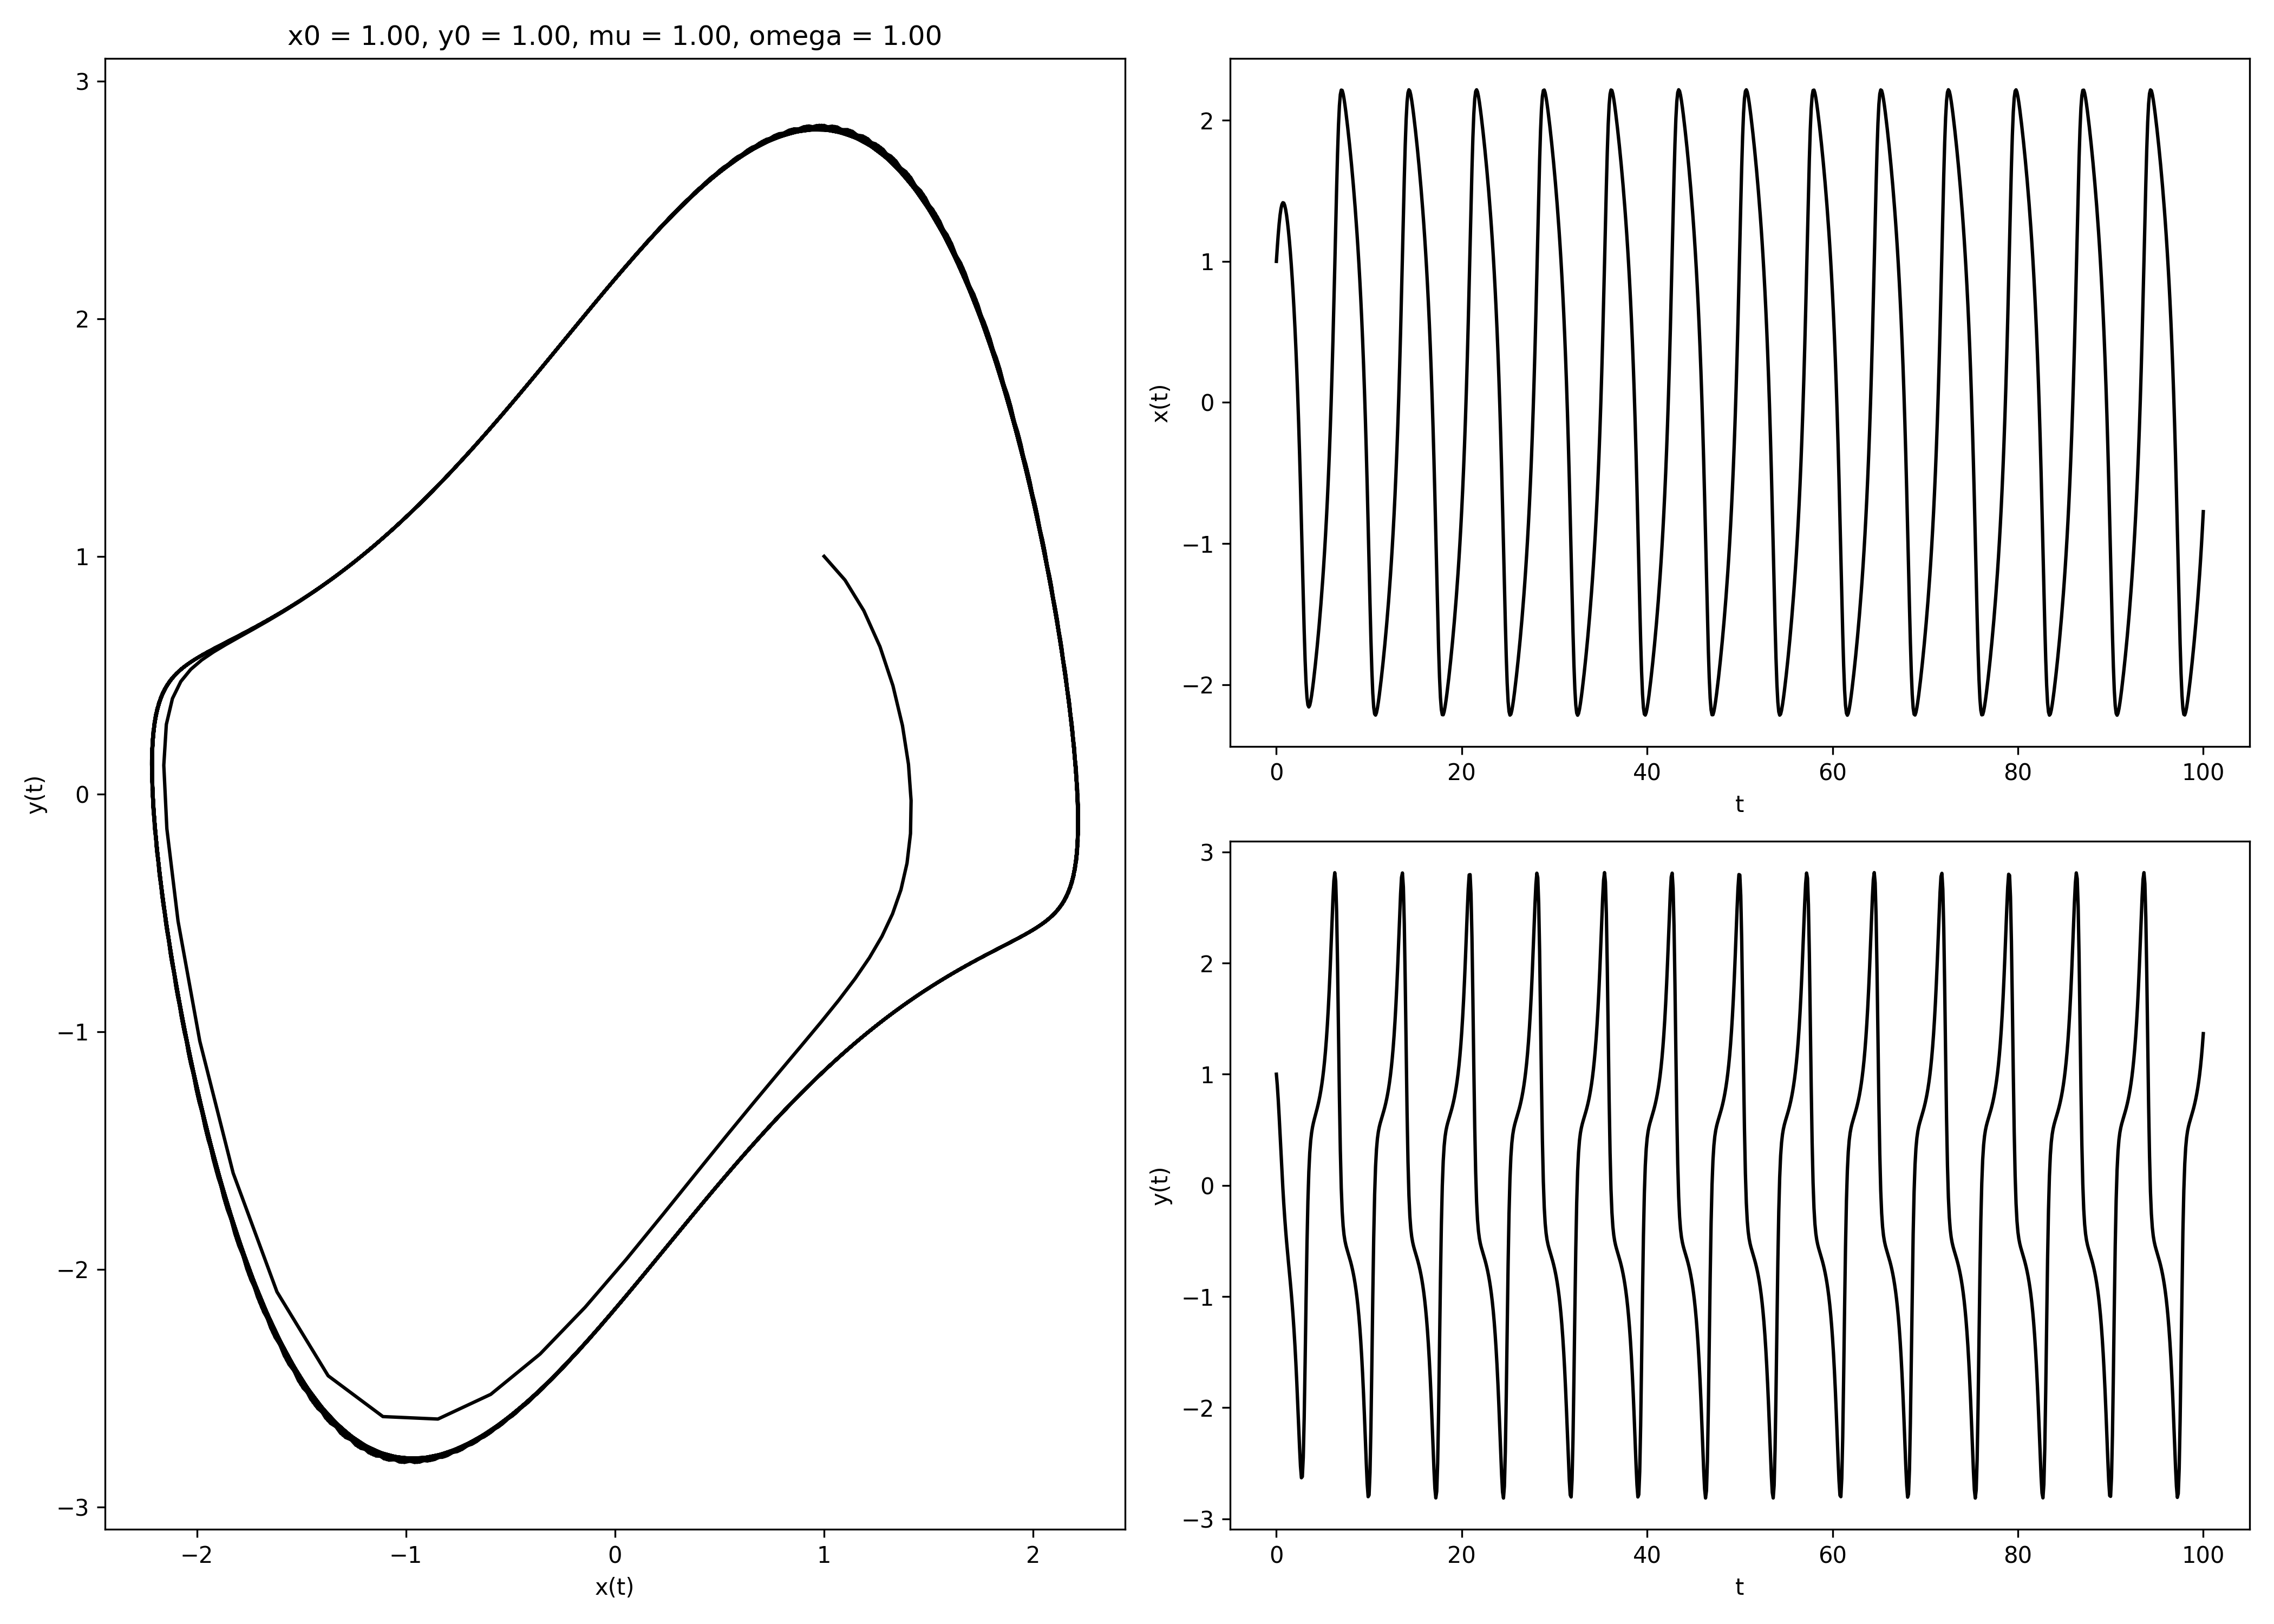
\includegraphics[draft, scale=0.33]{x1_0y1_0mu1_0omega1_0.png}
\figcaption{$x_0=1.00, y_0=1.00, \mu=1.00, \omega=1.00$}
%パラメーターmu
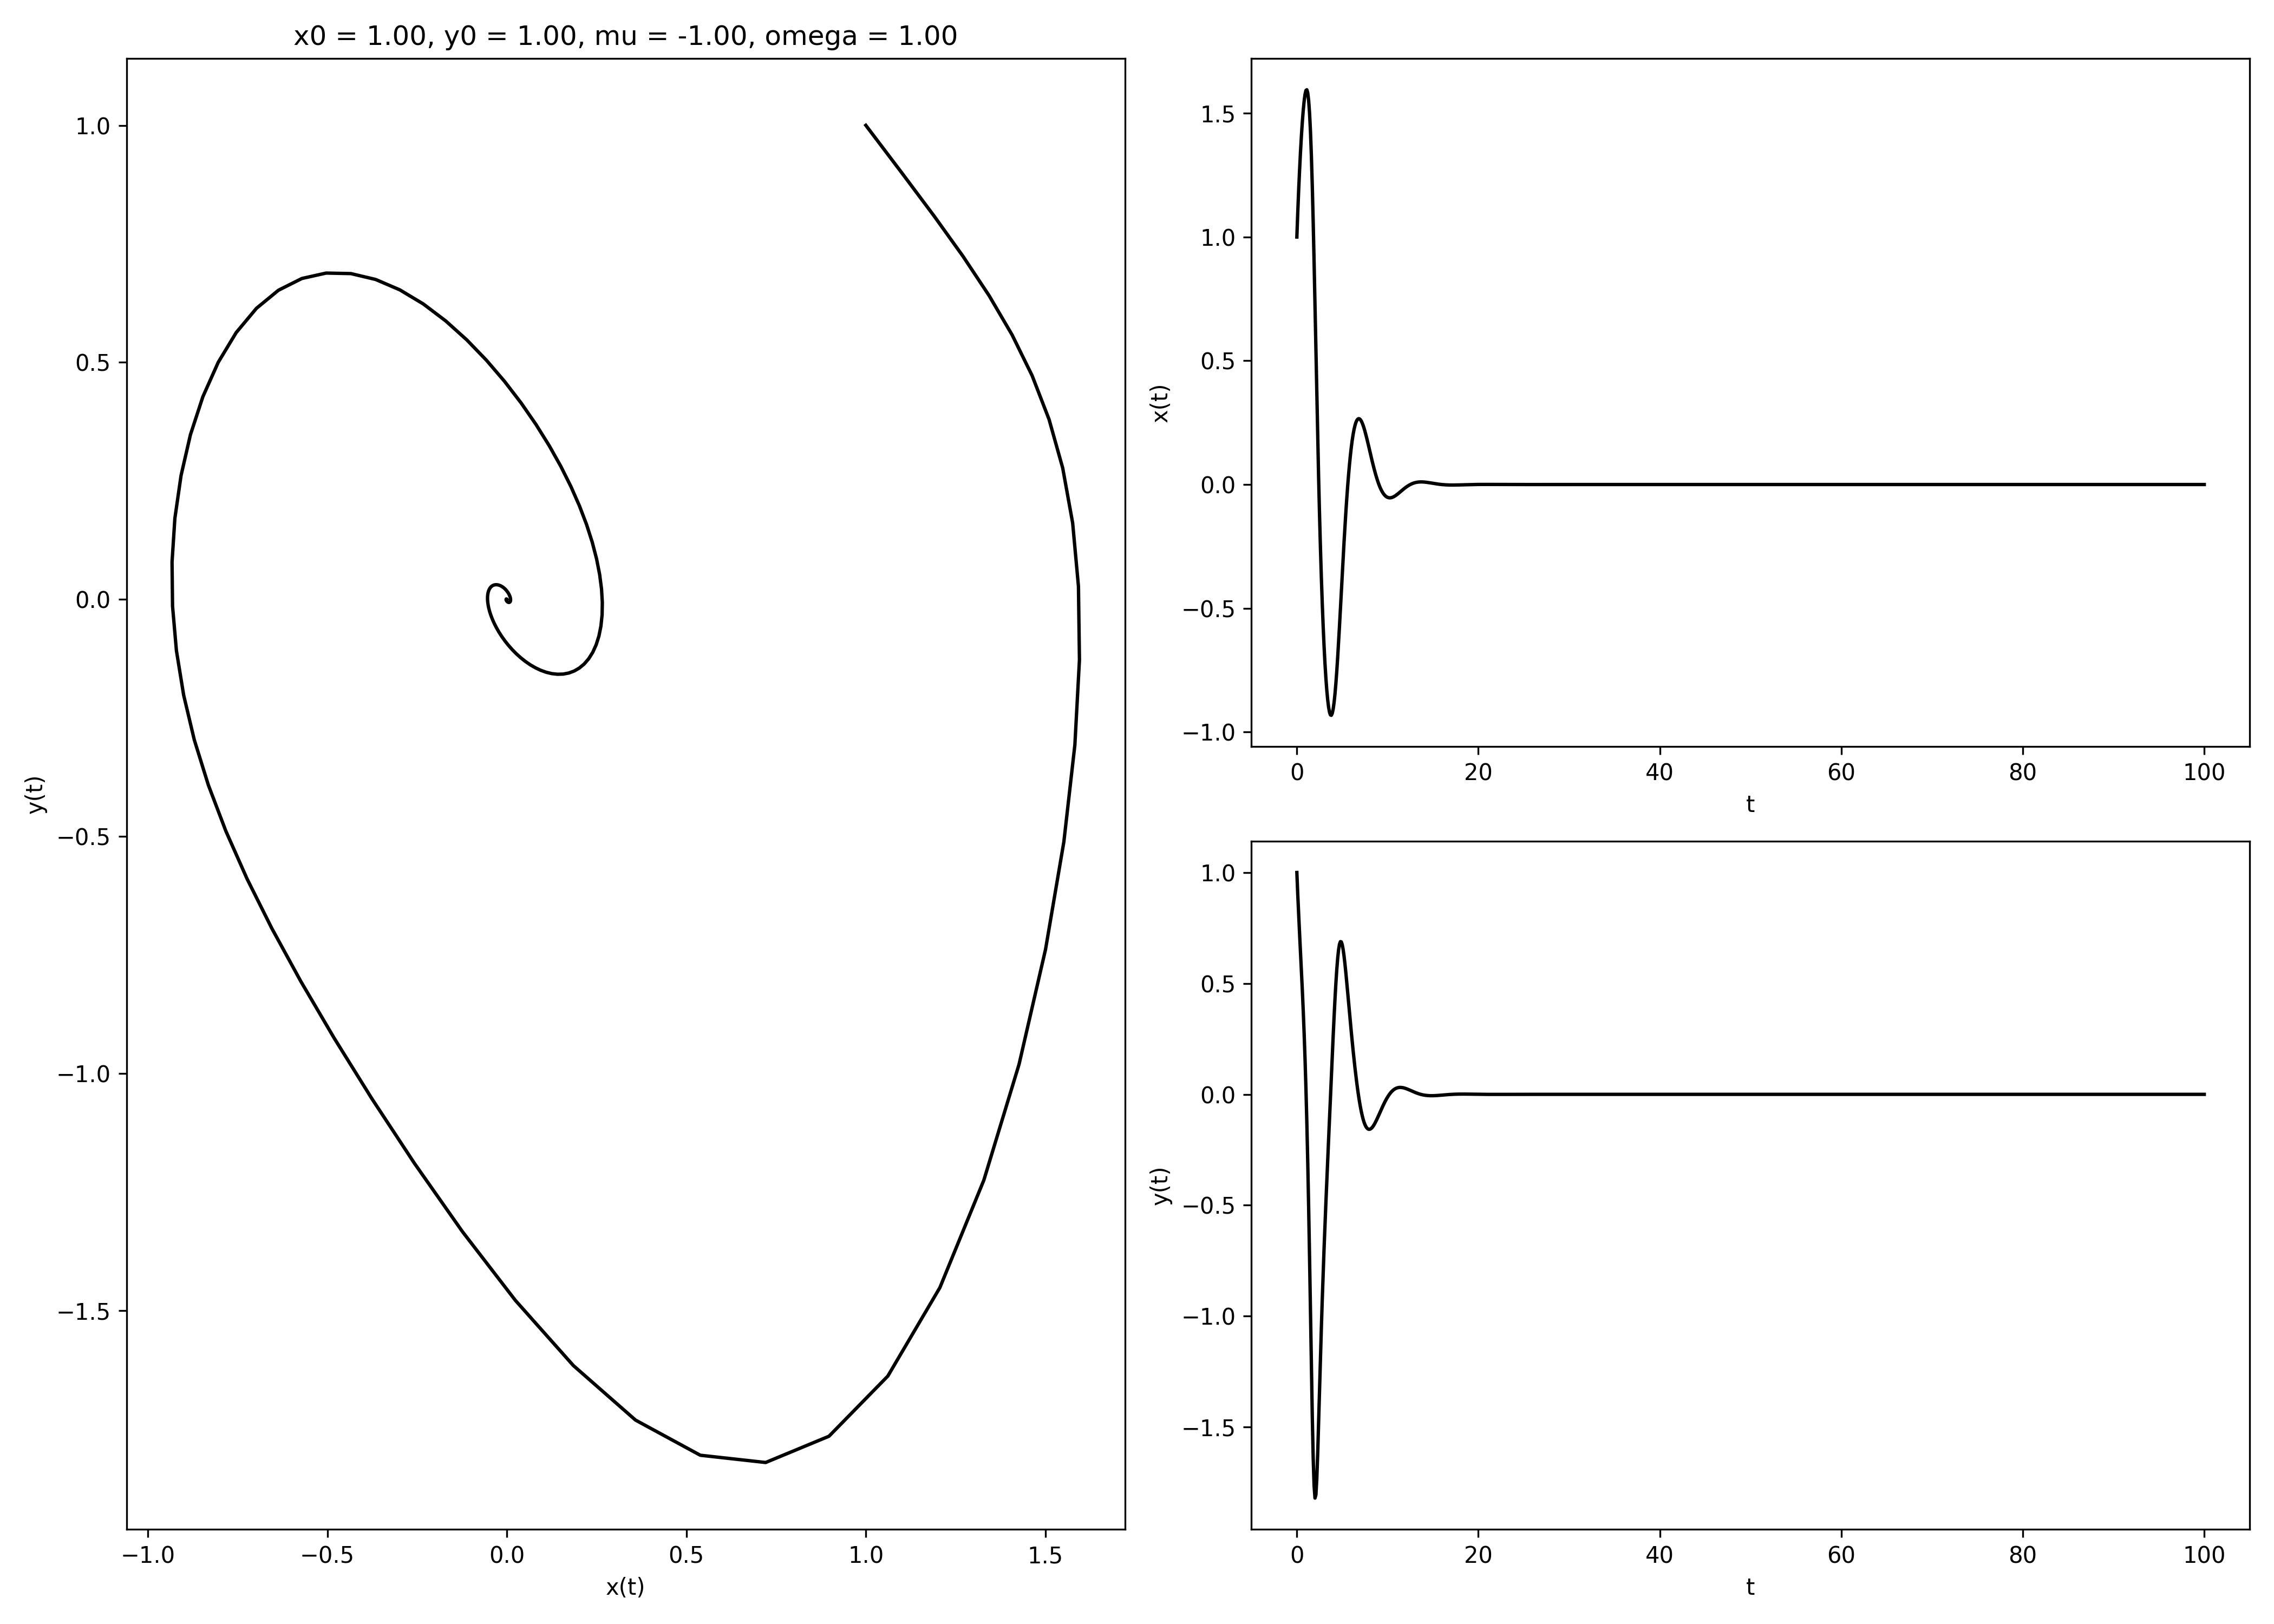
\includegraphics[draft, scale=0.33]{x1_0y1_0mu-1_0omega1_0.png}
\figcaption{$x_0=1.00, y_0=1.00, \mu=-1.00, \omega=1.00$}
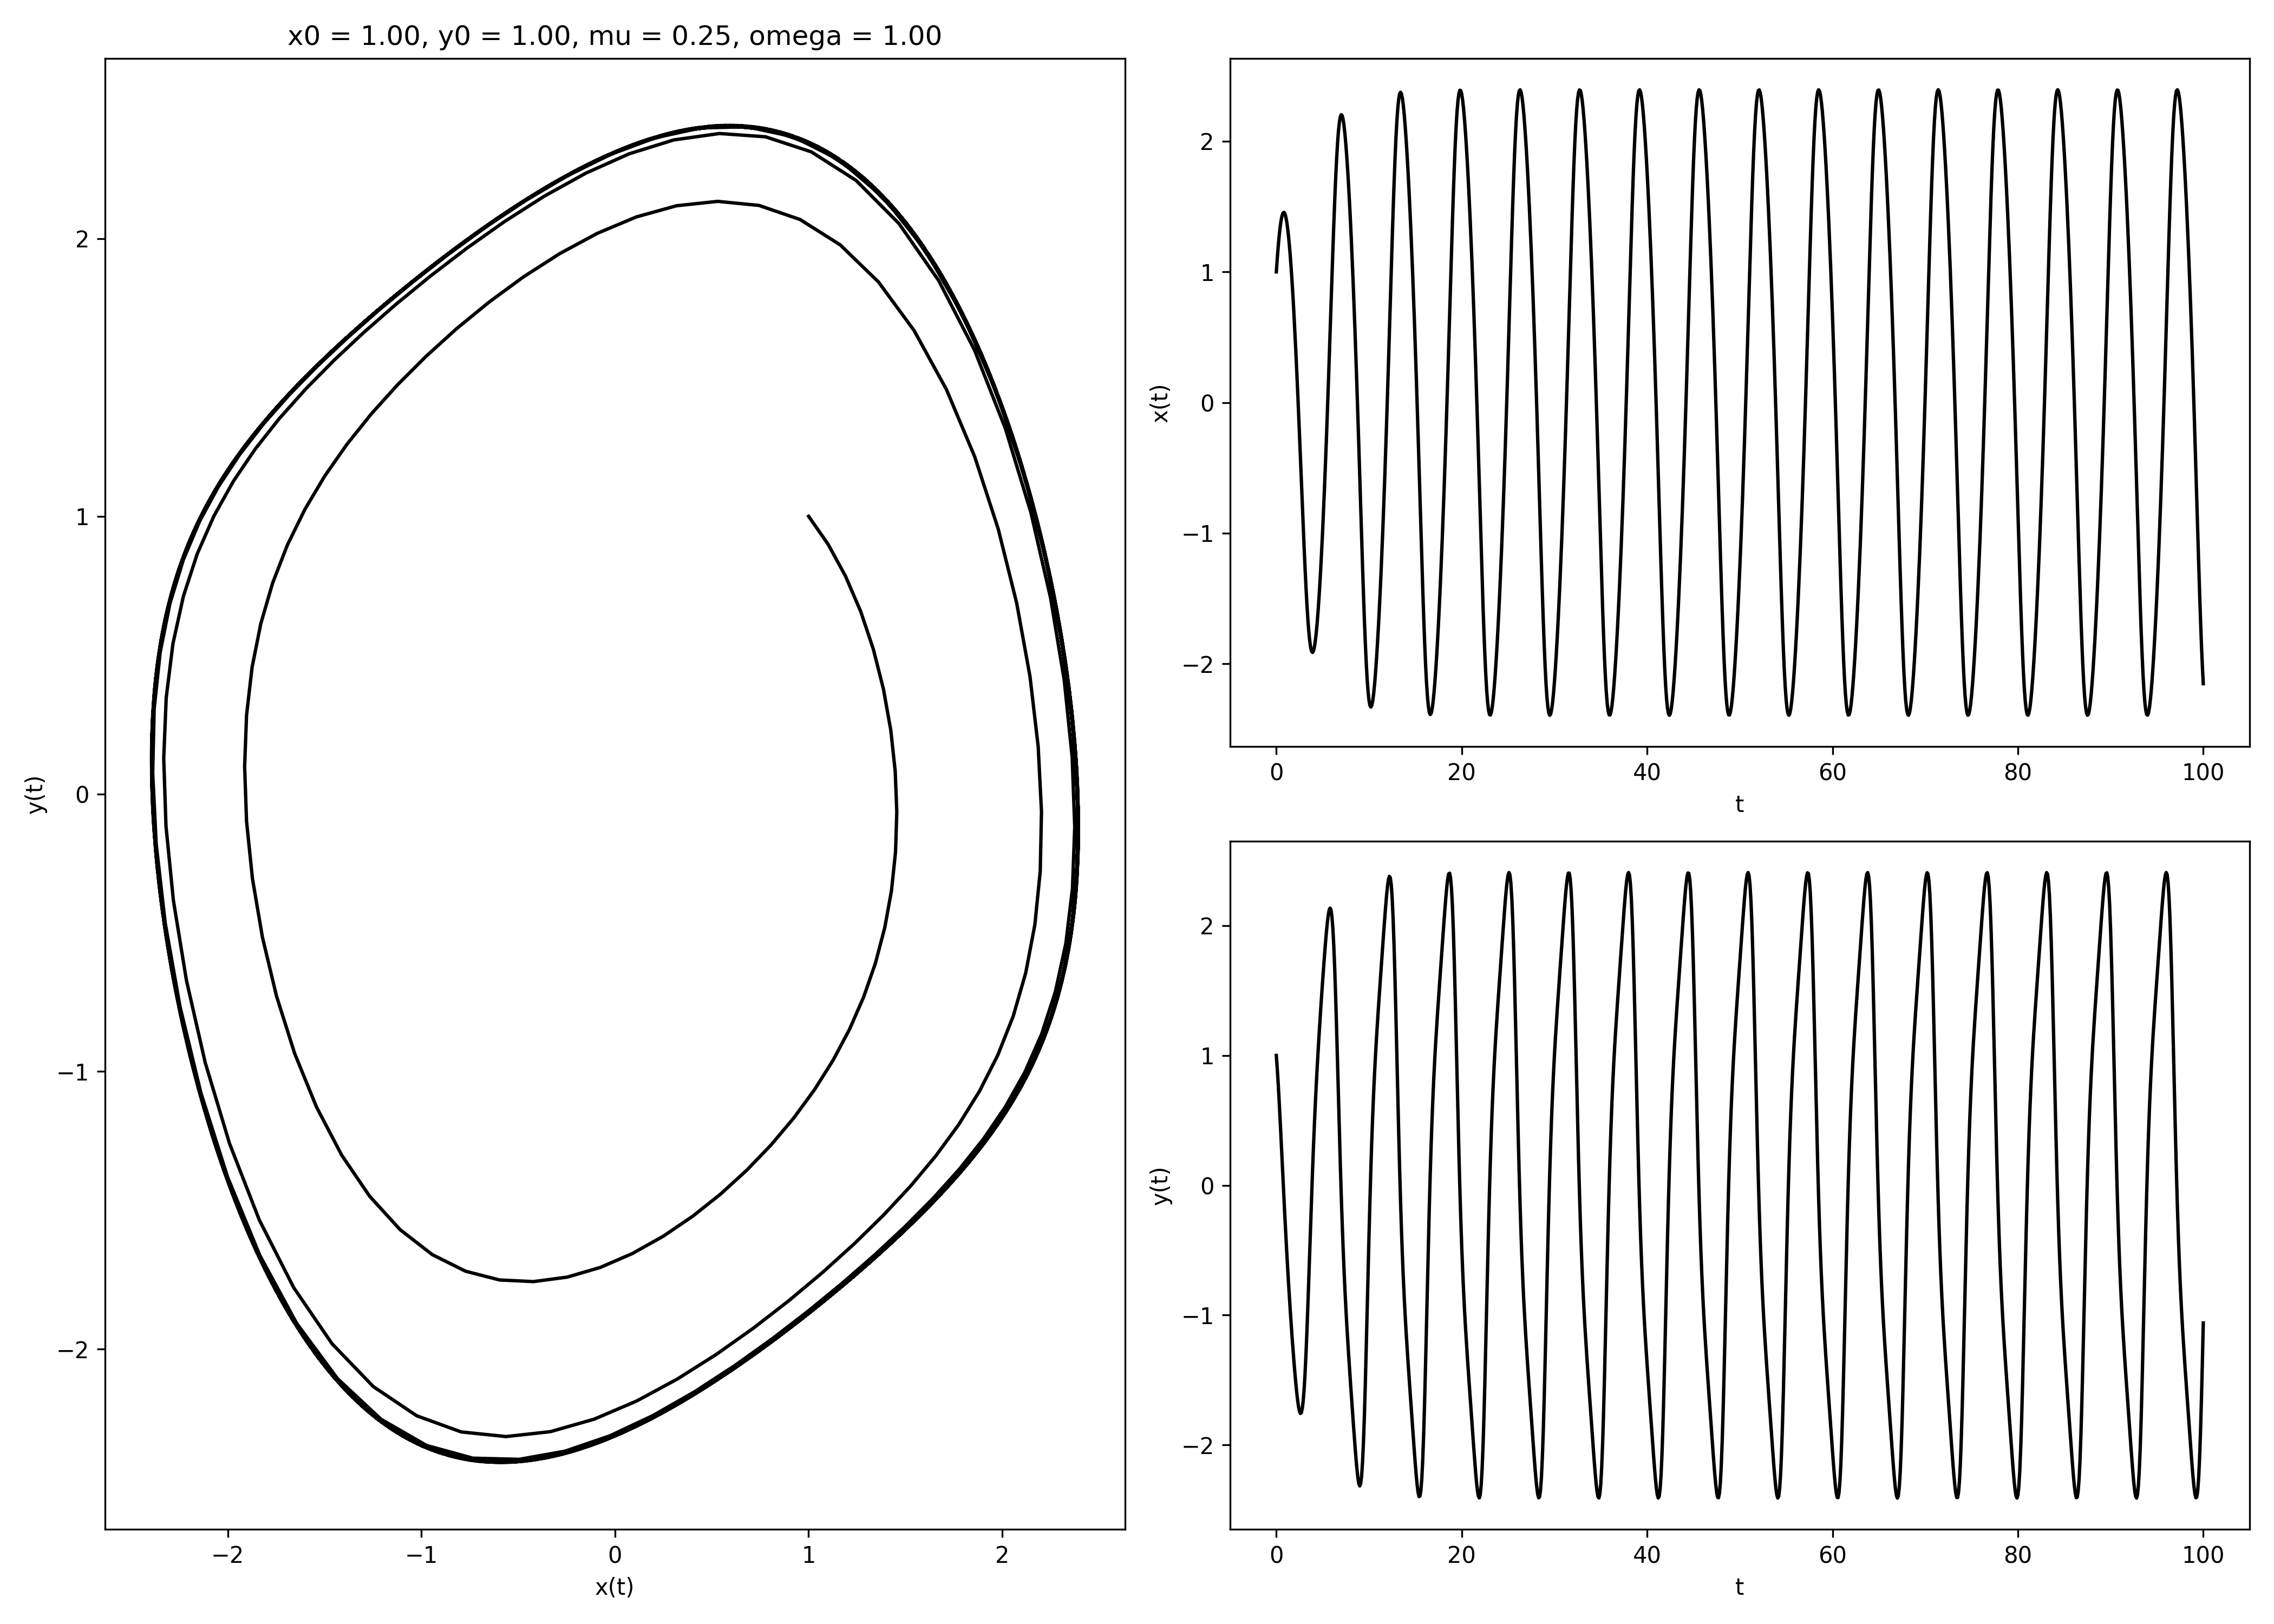
\includegraphics[draft, scale=0.33]{x1_0y1_0mu0_2omega1_0.png}
\figcaption{$x_0=1.00, y_0=1.00, \mu=0.25, \omega=1.00$}
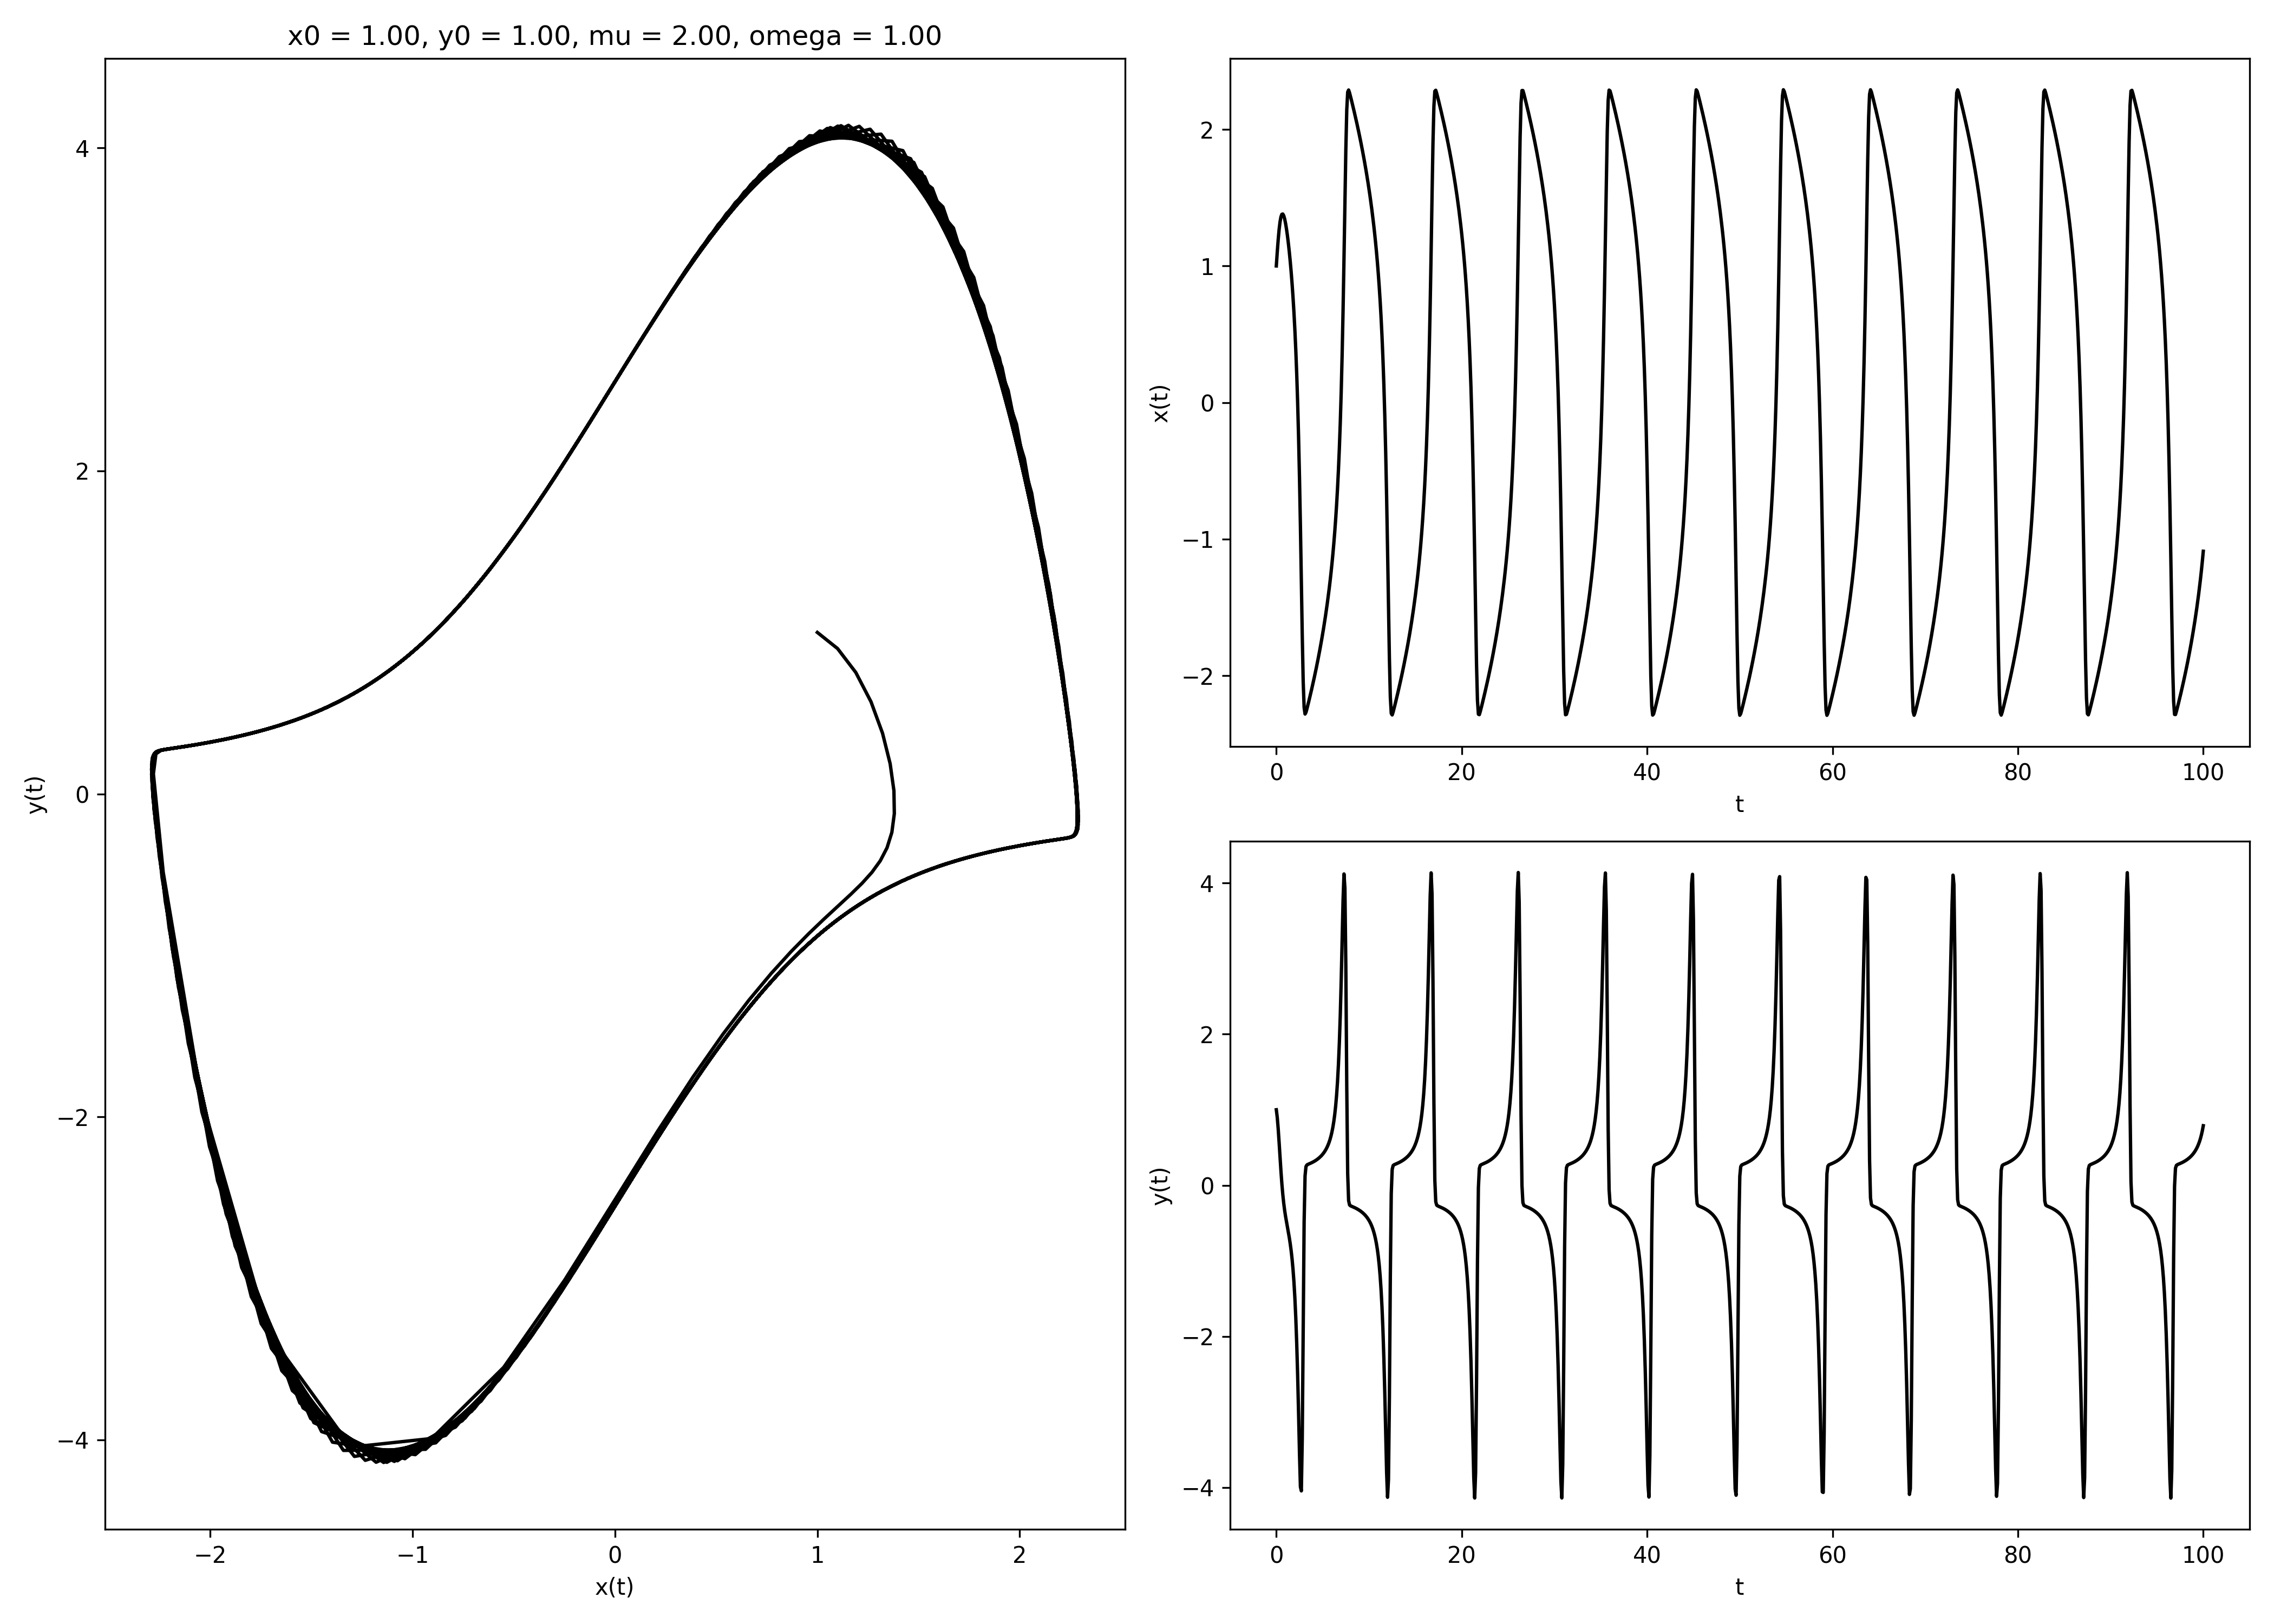
\includegraphics[draft, scale=0.33]{x1_0y1_0mu2_0omega1_0.png}
\figcaption{$x_0=1.00, y_0=1.00, \mu=2.00, \omega=1.00$}
%パラメーターomega
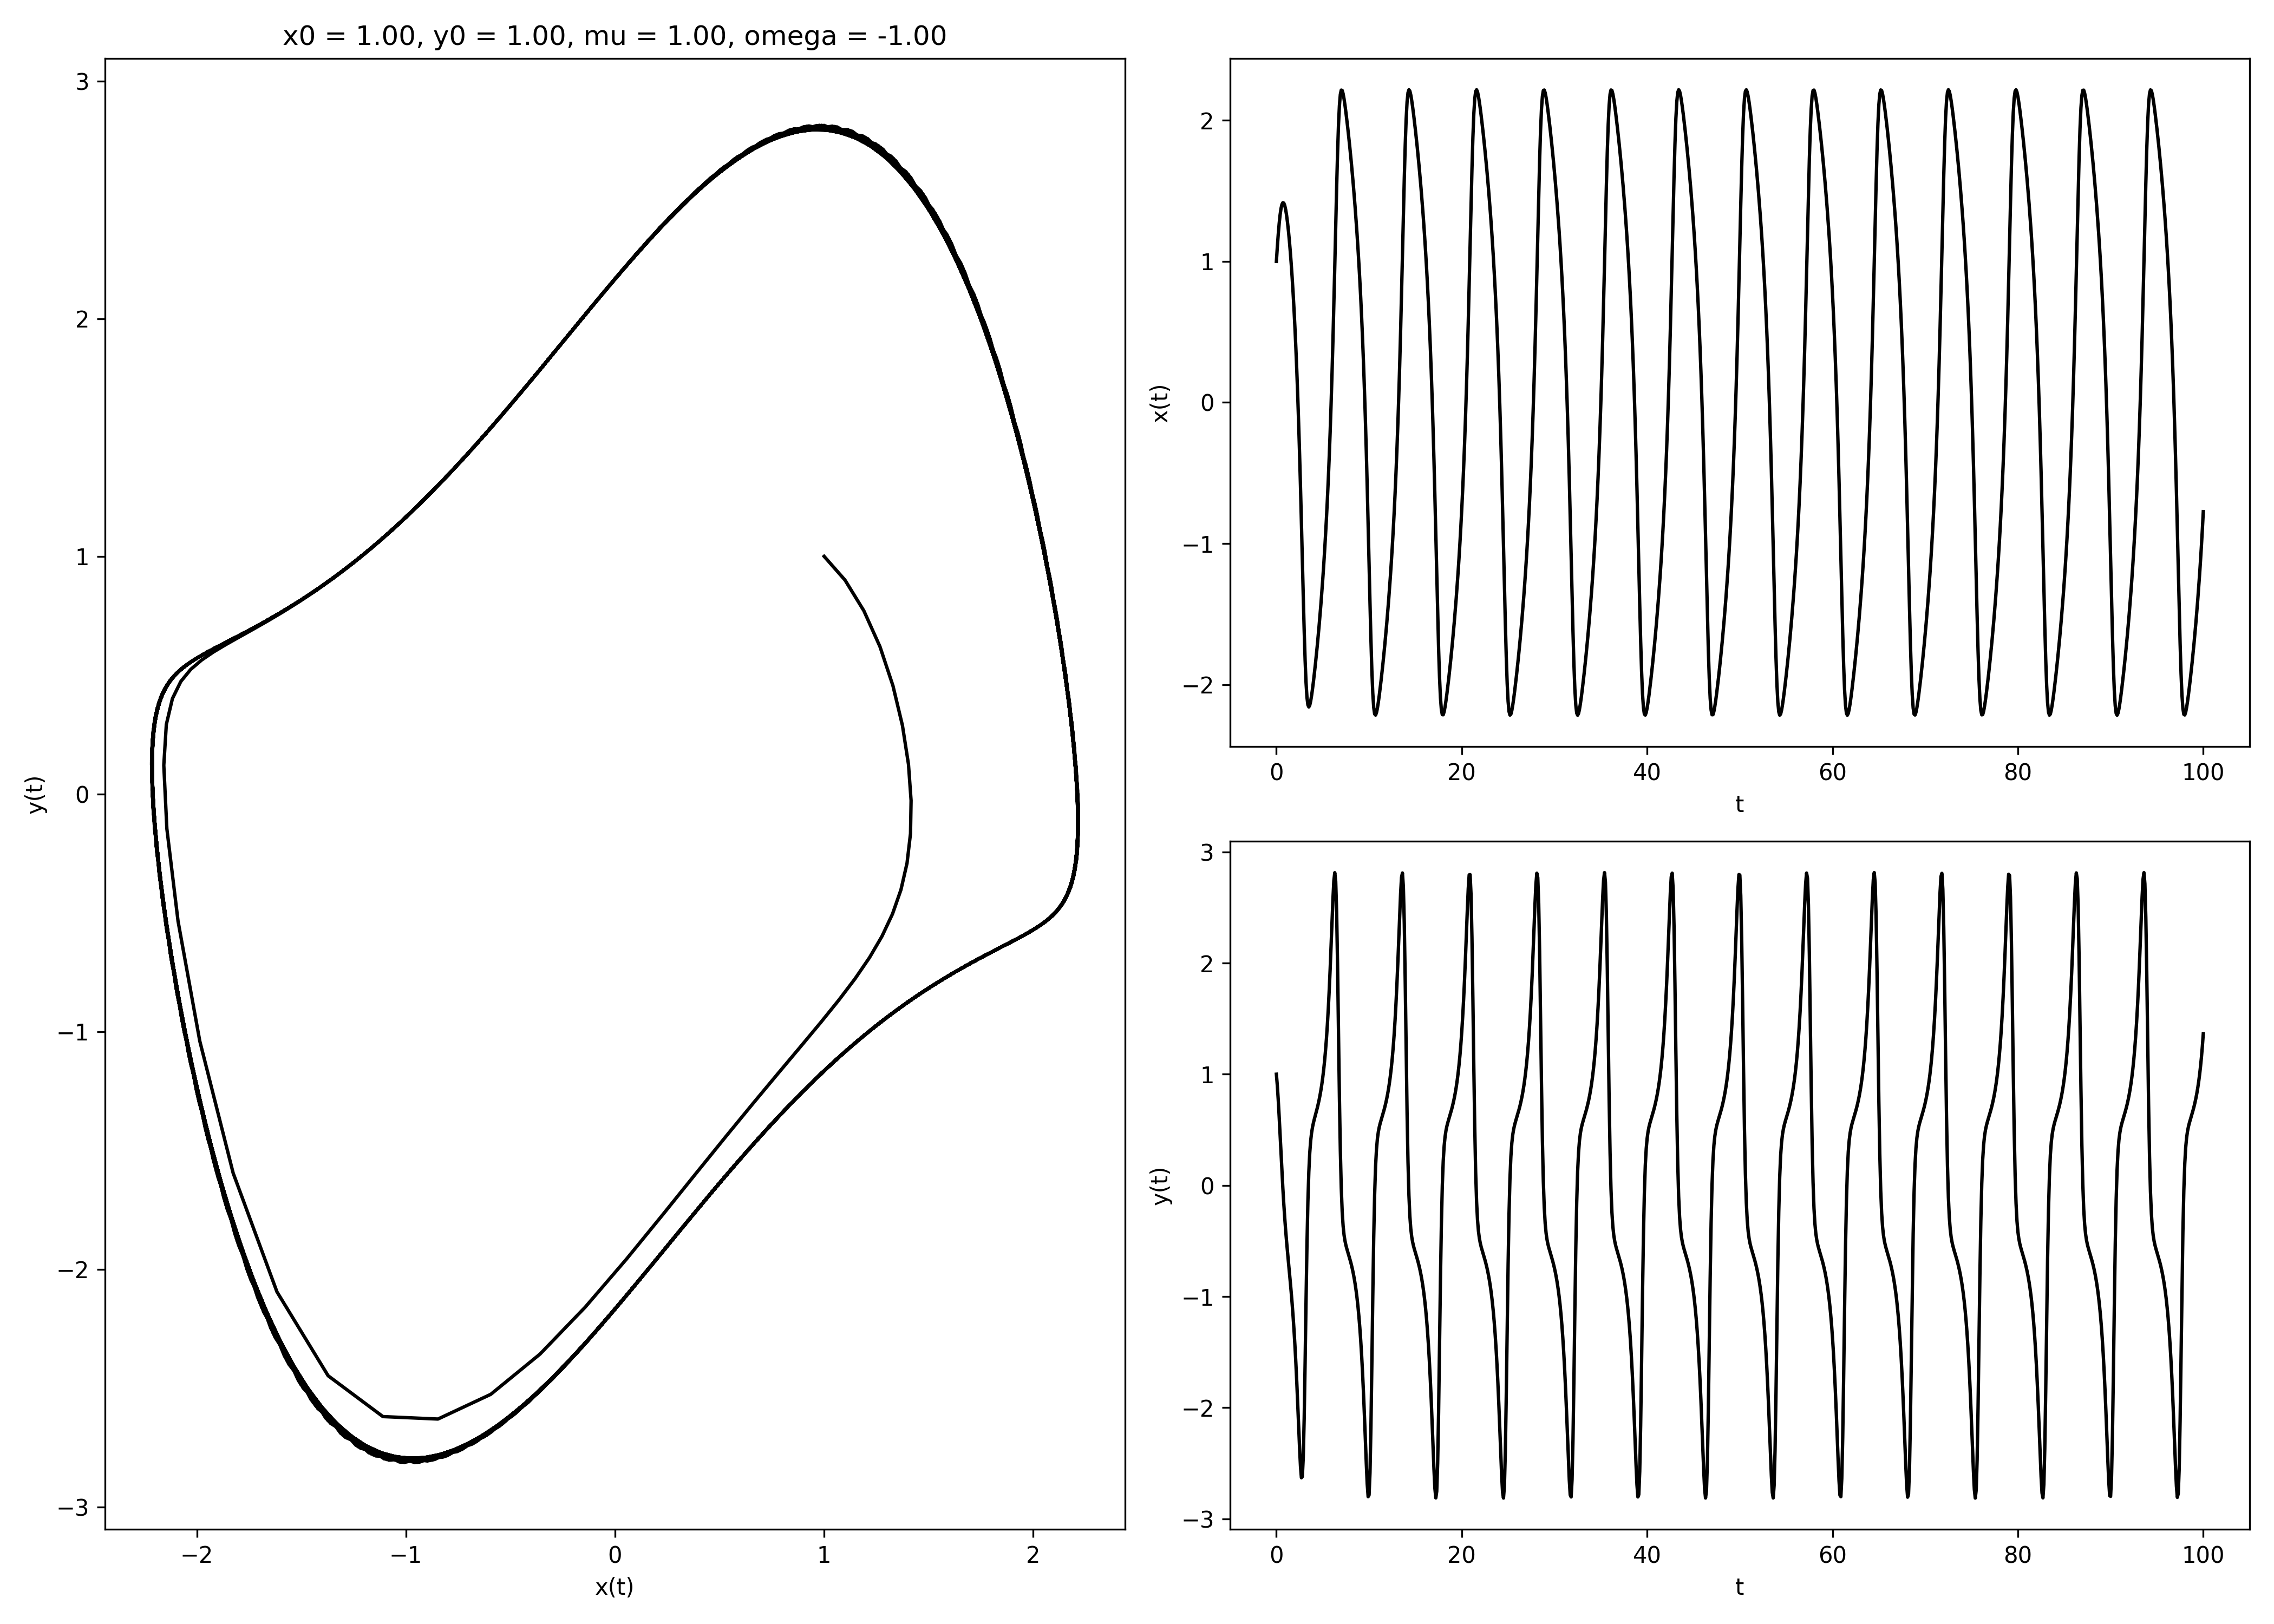
\includegraphics[draft, scale=0.33]{x1_0y1_0mu1_0omega-1_0.png}
\figcaption{$x_0=1.00, y_0=1.00, \mu=1.00, \omega=-1.00$}
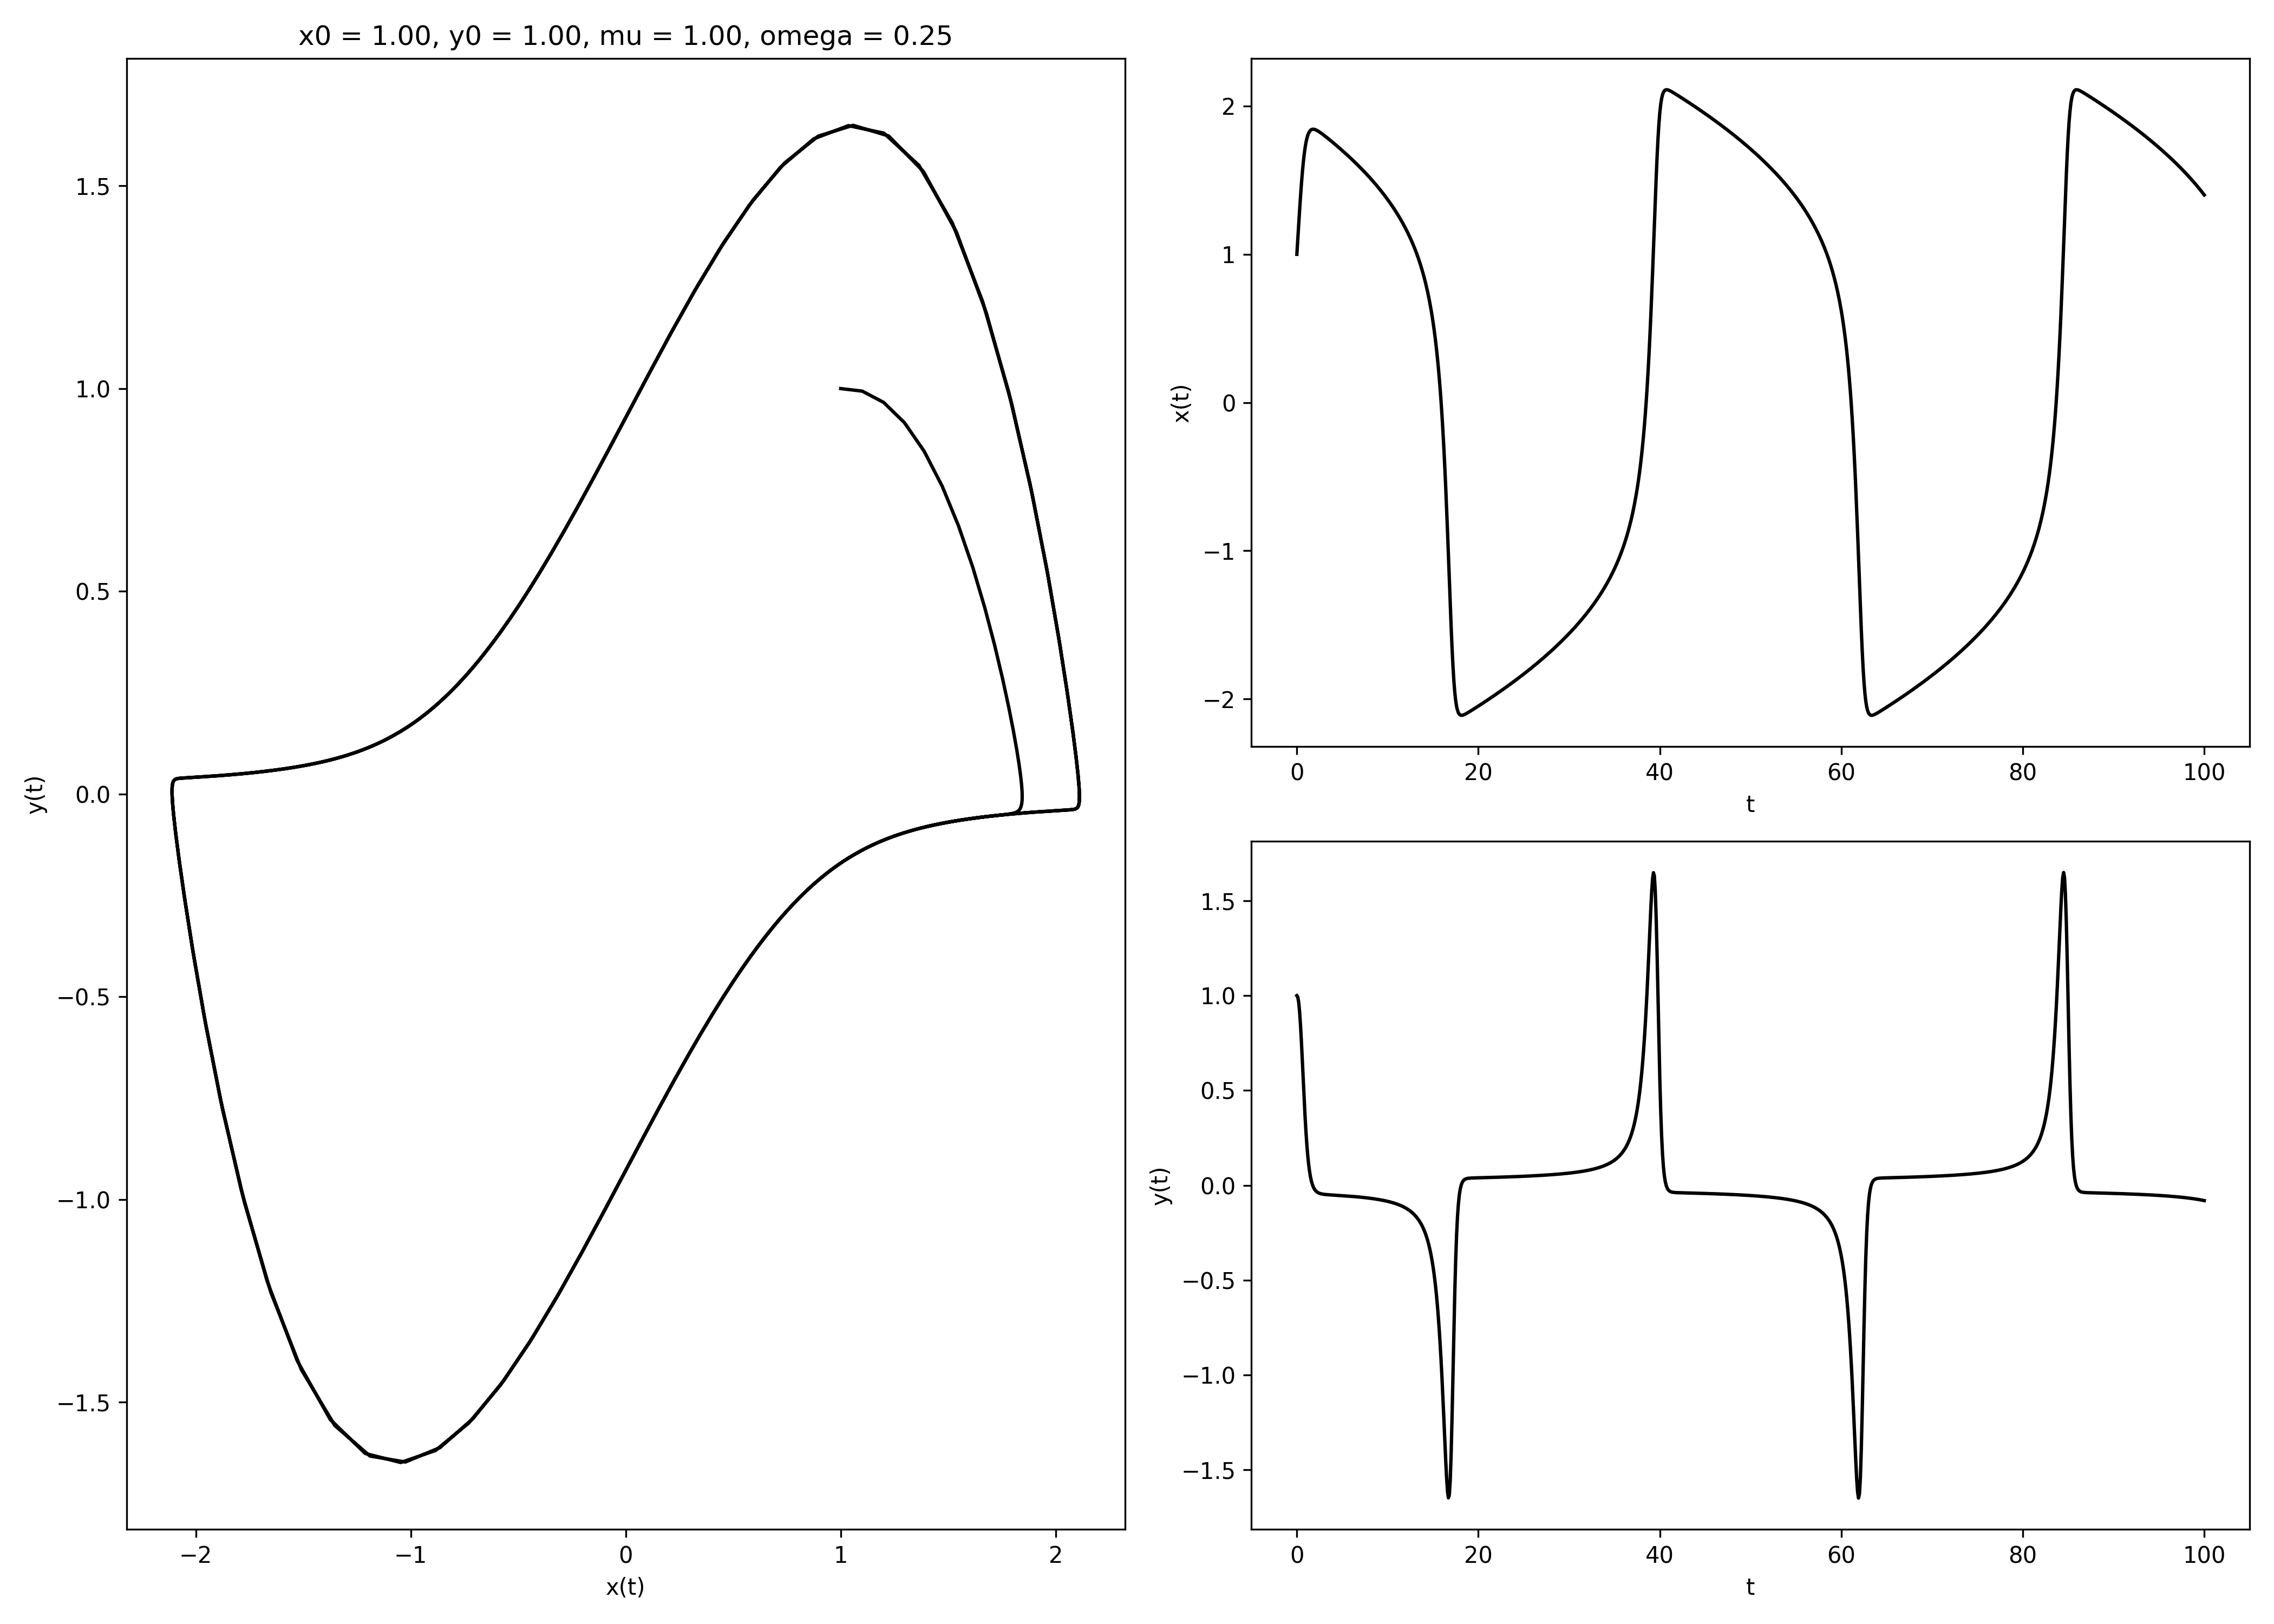
\includegraphics[draft, scale=0.33]{x1_0y1_0mu1_0omega0_2.png}
\figcaption{$x_0=1.00, y_0=1.00, \mu=1.00, \omega=0.25$}
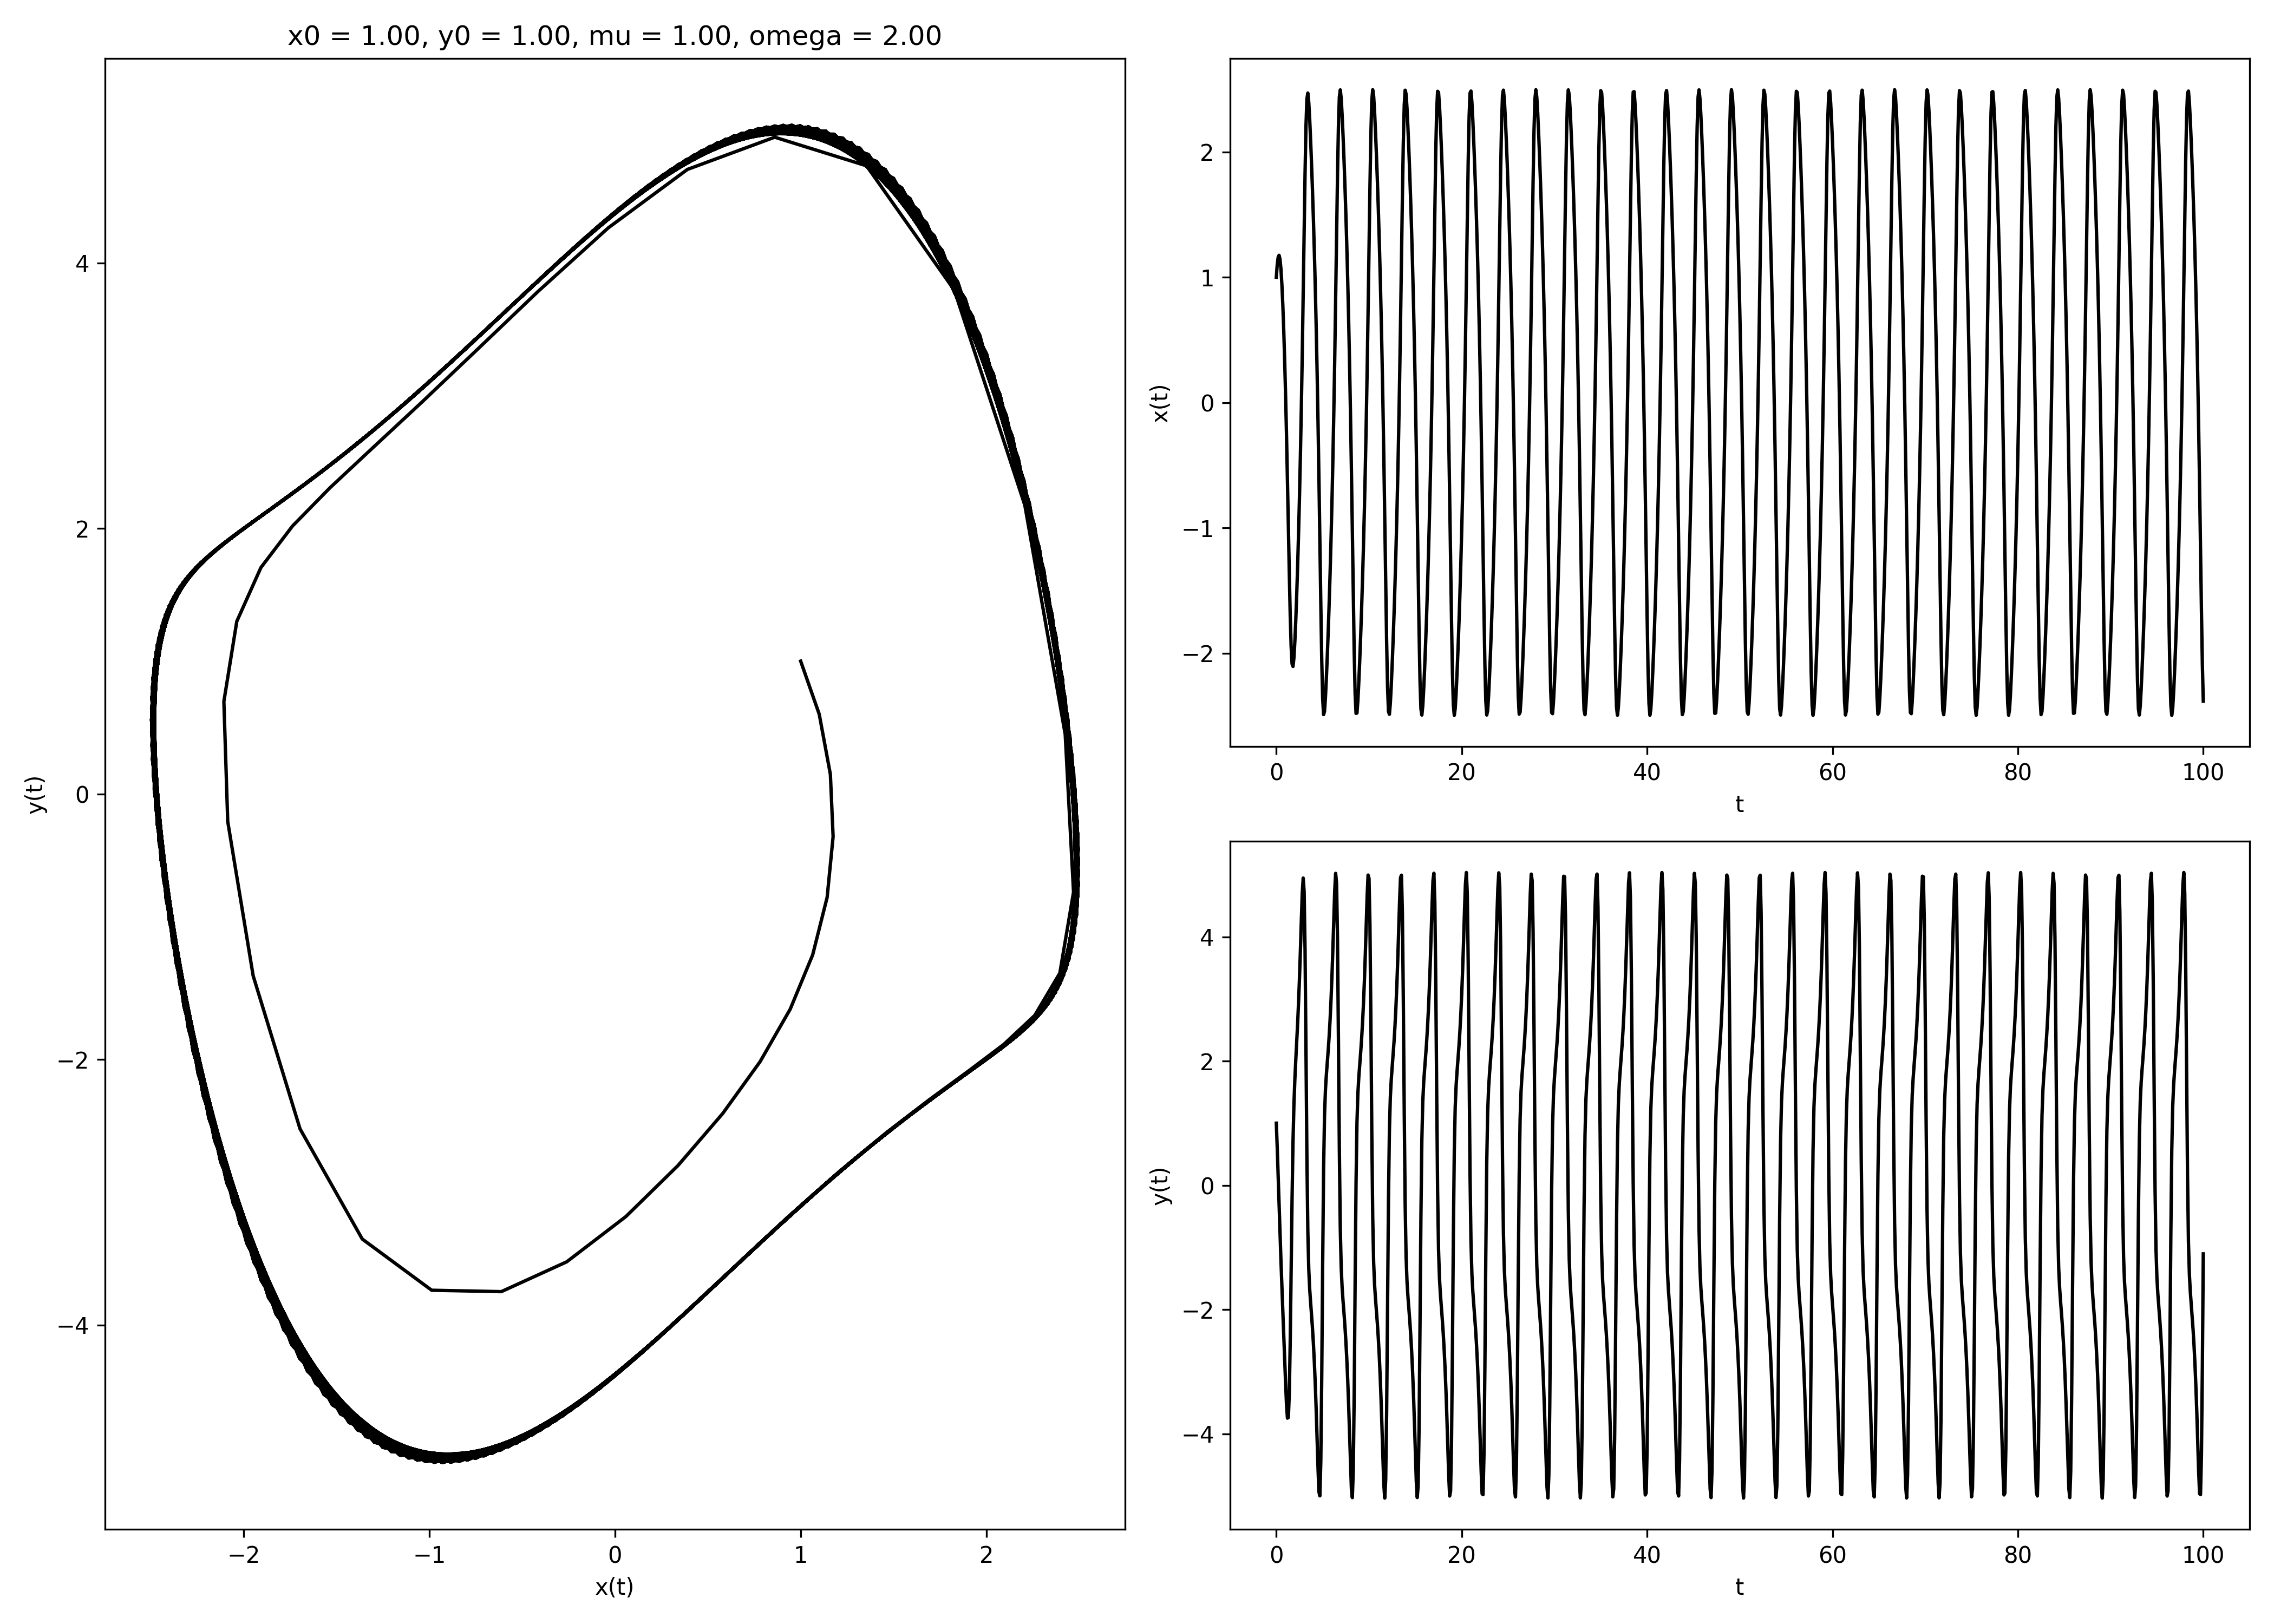
\includegraphics[draft, scale=0.33]{x1_0y1_0mu1_0omega2_0.png}
\figcaption{$x_0=1.00, y_0=1.00, \mu=1.00, \omega=2.00$}
%パラメーター初期値
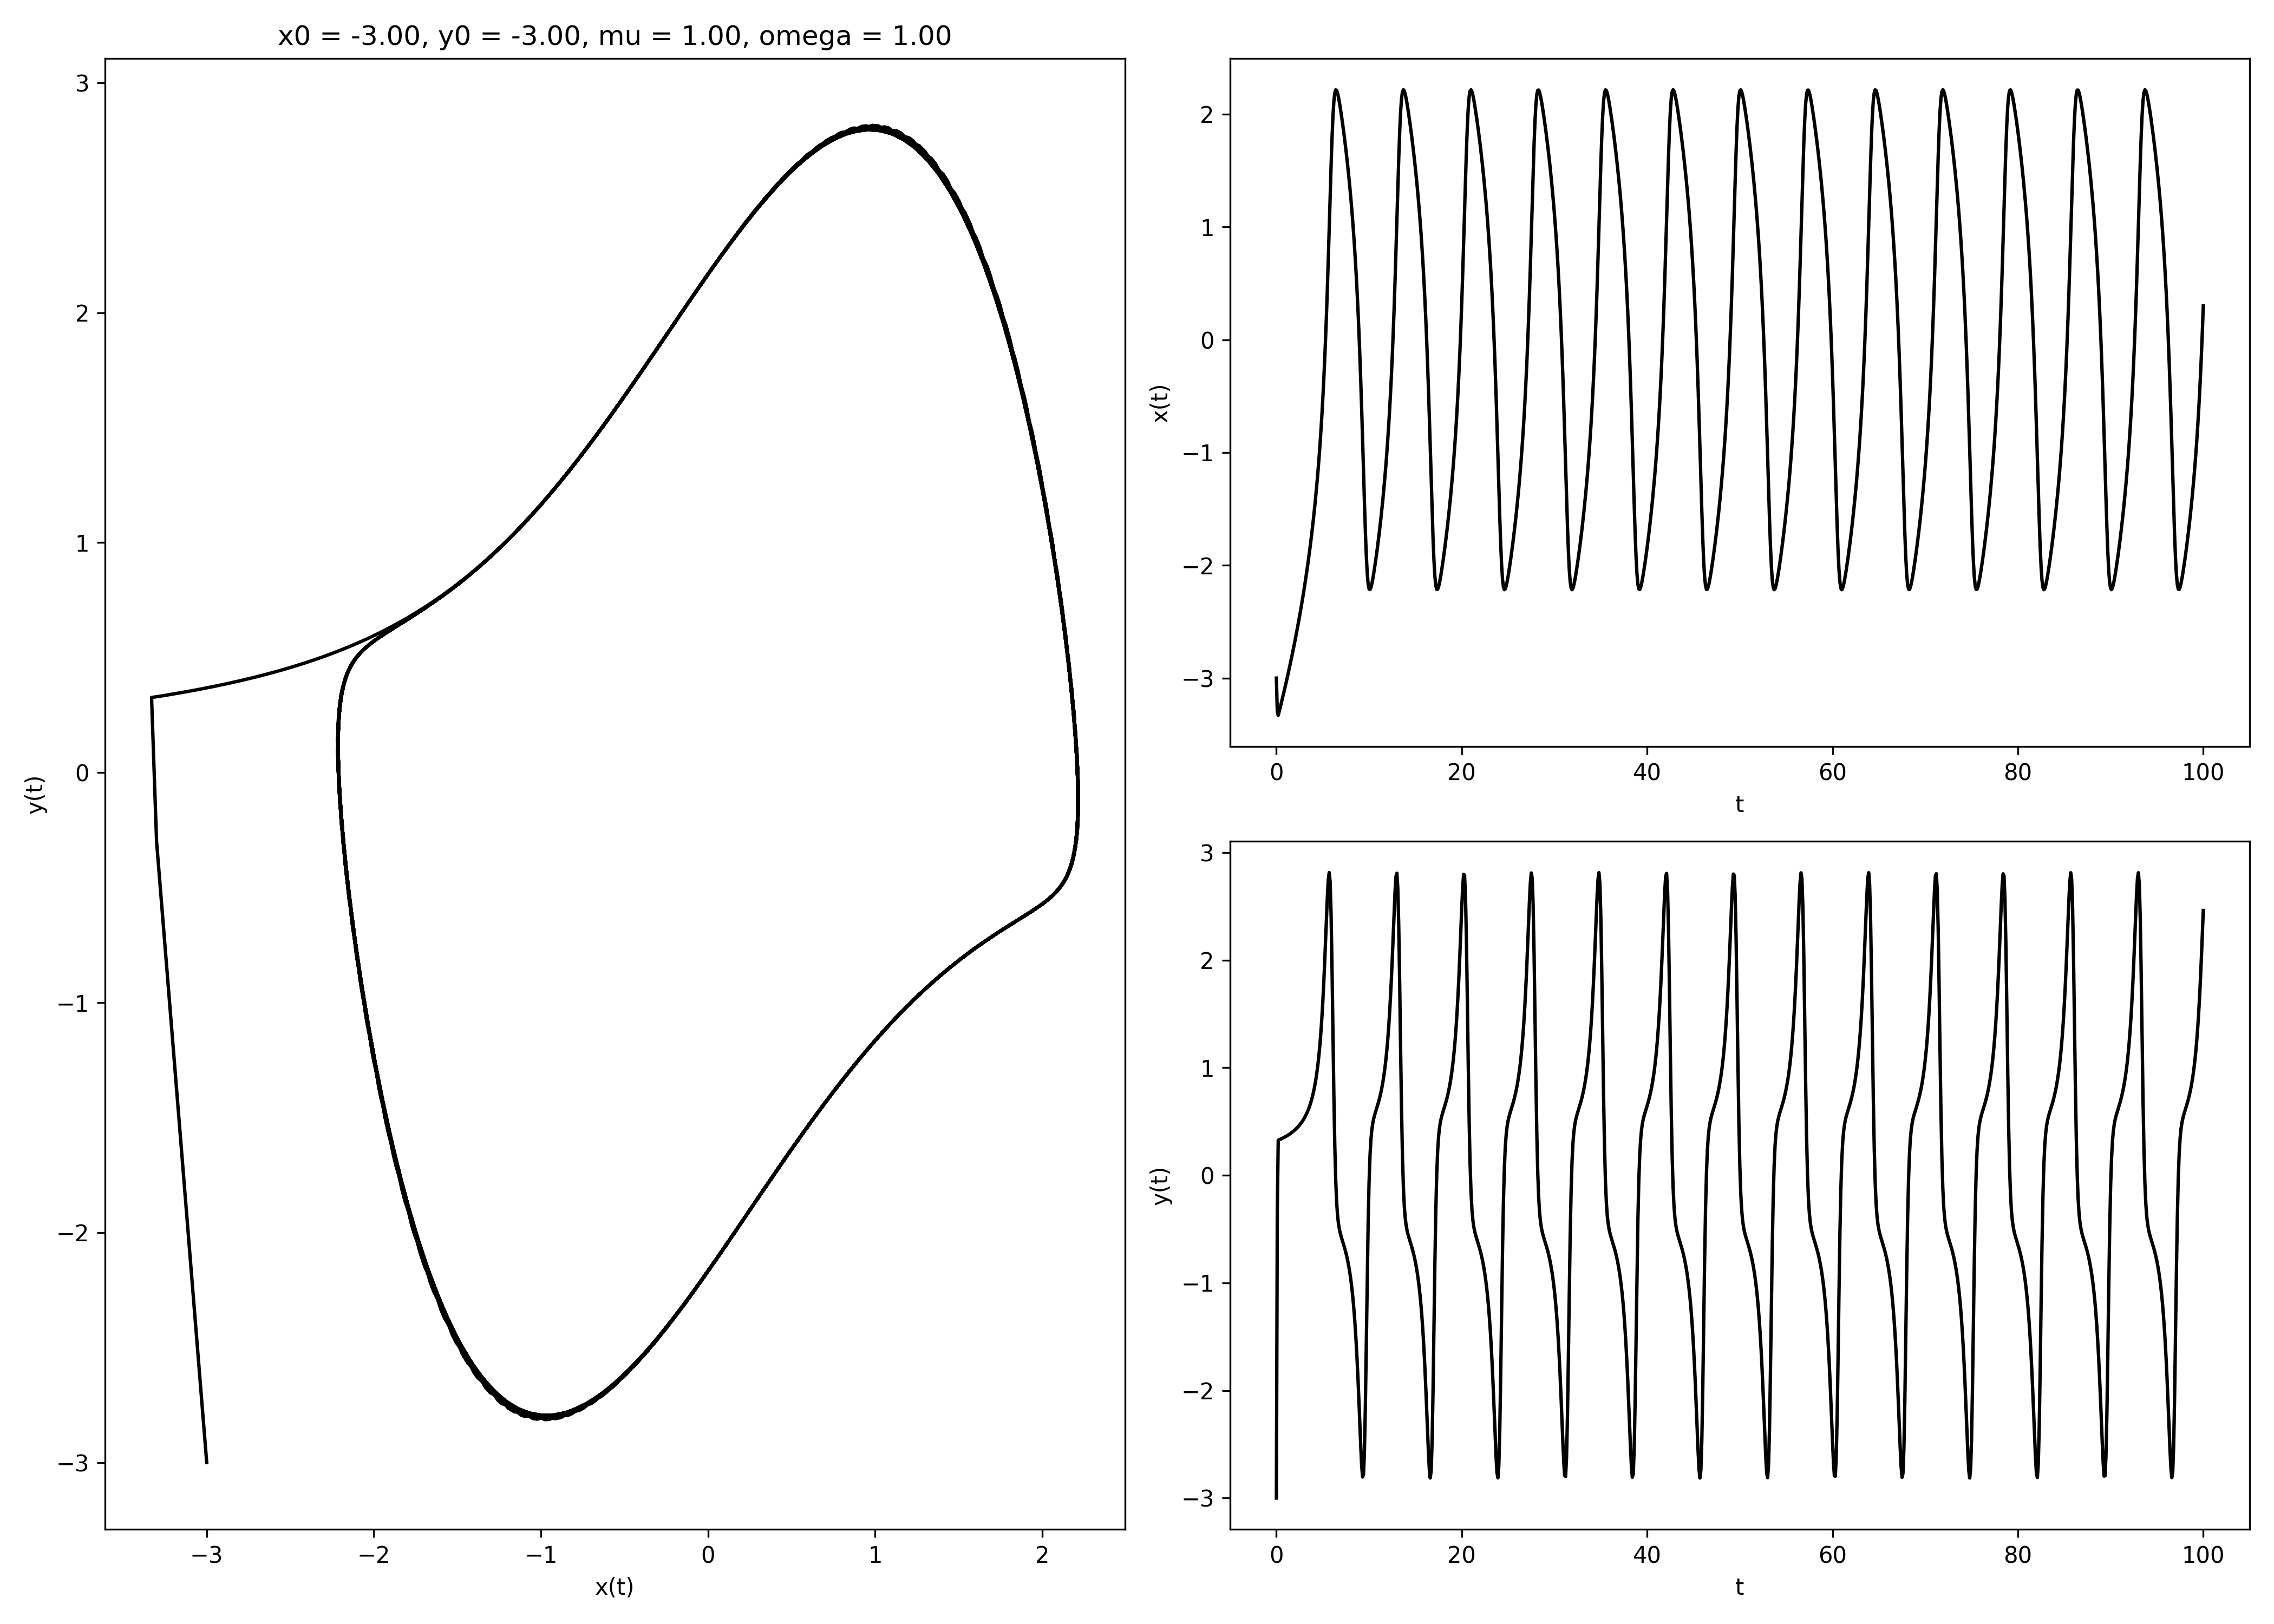
\includegraphics[draft, scale=0.33]{x-3_0y-3_0mu1_0omega1_0.png}
\figcaption{$x_0=-3.00, y_0=-3.00, \mu=1.00, \omega=1.00$}
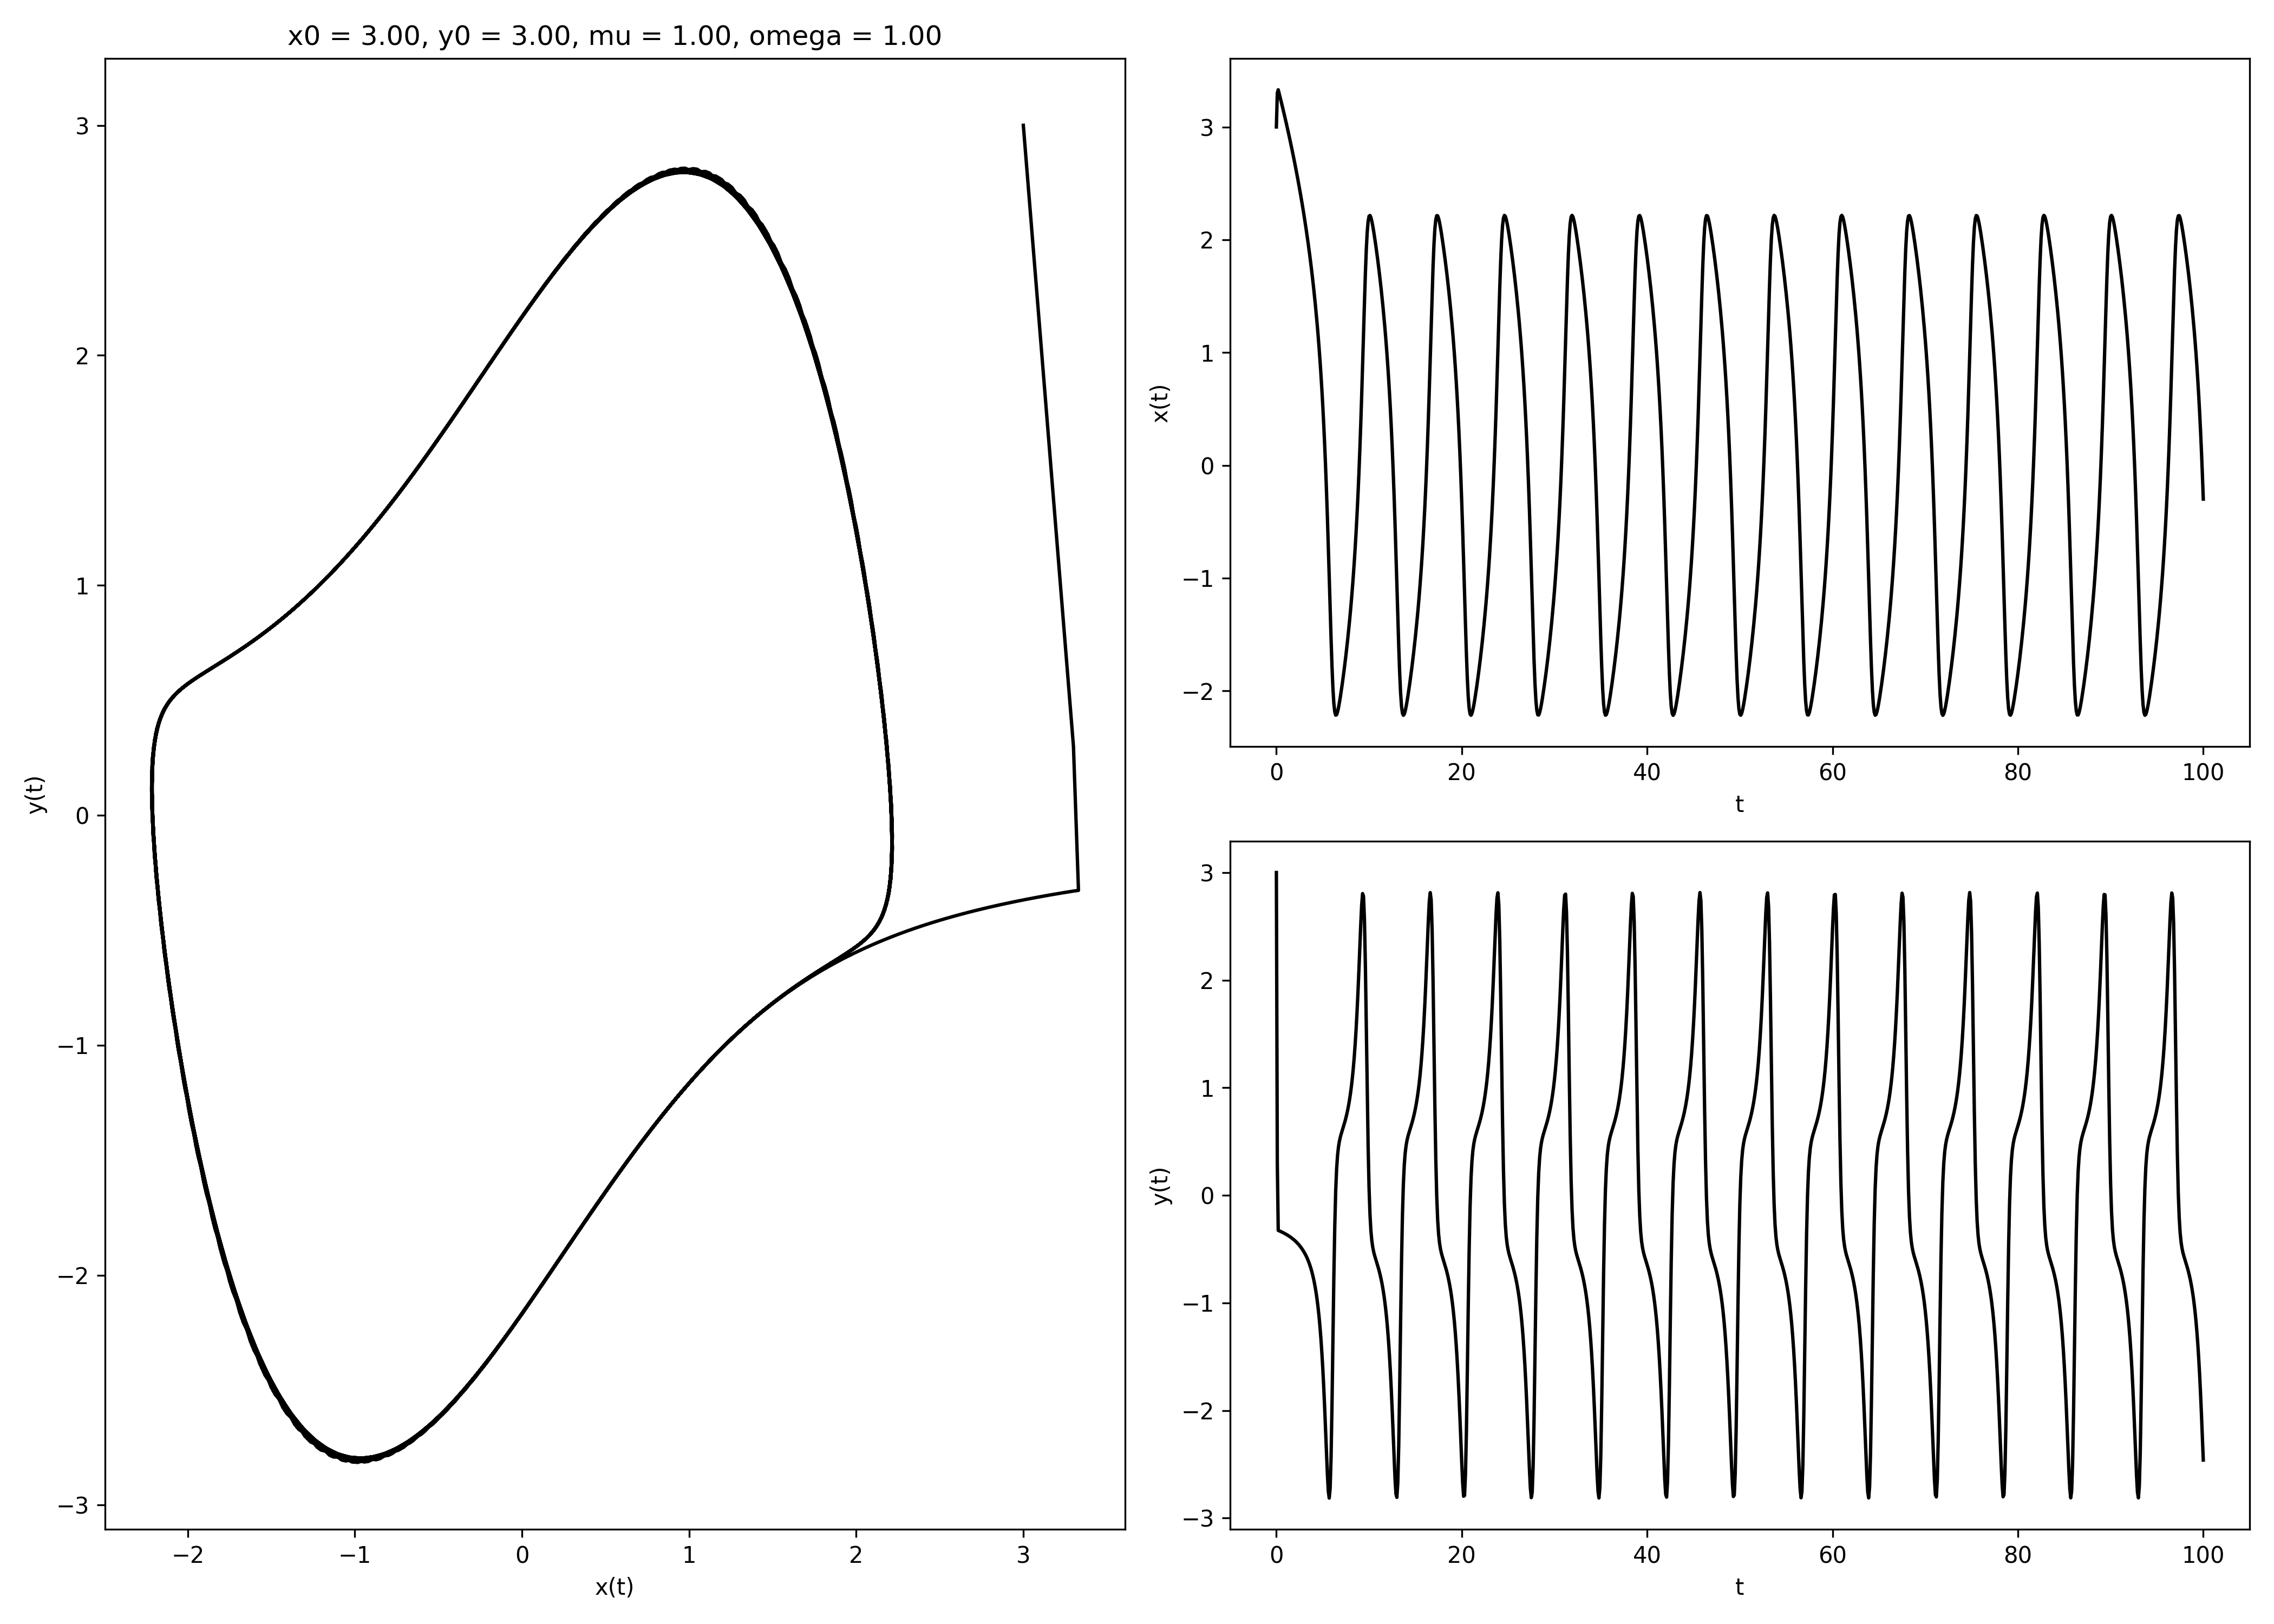
\includegraphics[draft, scale=0.33]{x3_0y3_0mu1_0omega1_0.png}
\figcaption{$x_0=3.00, y_0=3.00, \mu=1.00, \omega=1.00$}

%-----------------------考察---------------------
\section{考察}
\subsection{van der Pol 方程式}
初期値$(x_0, y_0)$によっての影響はあまりないと考えられた. しかし$(\mu, \omega)$に対して方程式が変化すると思われる. $\mu$については
\textbf{Limit cycle}(リミットサイクル)と呼ばれる周期軌道に収束した.


\section{結論}
\section{参考文献}
\section{感想}






\end{document}
